\subsection{Symbolic execution}
\label{symbolic_exec}

\subsubsection{Swapping two values using XOR}

There is a well-known (but counterintuitive) algorithm for swapping two values in two variables
using XOR operation without use of any additional memory/register:

\begin{lstlisting}
X=X^Y
Y=Y^X
X=X^Y
\end{lstlisting}

How it works?
It would be better to construct an expression at each step of execution.

\lstinputlisting{symbolic/1_XOR/xor_swap.py}

It works, because Python is dynamicaly typed \ac{PL}, so the function doesn't care what to operate on,
numerical values, or on objects of Expr() class.

Here is result:

\begin{lstlisting}
new_X ((X^Y)^(Y^(X^Y)))
new_Y (Y^(X^Y))
\end{lstlisting}

You can remove double variables in your mind (since XORing by a value twice will result in nothing).
At new\_X we can drop two X-es and two Y-es, and single Y will left.
At new\_Y we can drop two Y-es, and single X will left.

\subsubsection{Change endianness}

What does this code do?

\begin{lstlisting}
mov     eax, ecx
mov     edx, ecx
shl     edx, 16
and     eax, 0000ff00H
or      eax, edx
mov     edx, ecx
and     edx, 00ff0000H
shr     ecx, 16
or      edx, ecx
shl     eax, 8
shr     edx, 8
or      eax, edx
\end{lstlisting}

In fact, many reverse engineers play shell game a lot, keeping track of what is stored where, at each point of time.

\begin{figure}[H]
\centering
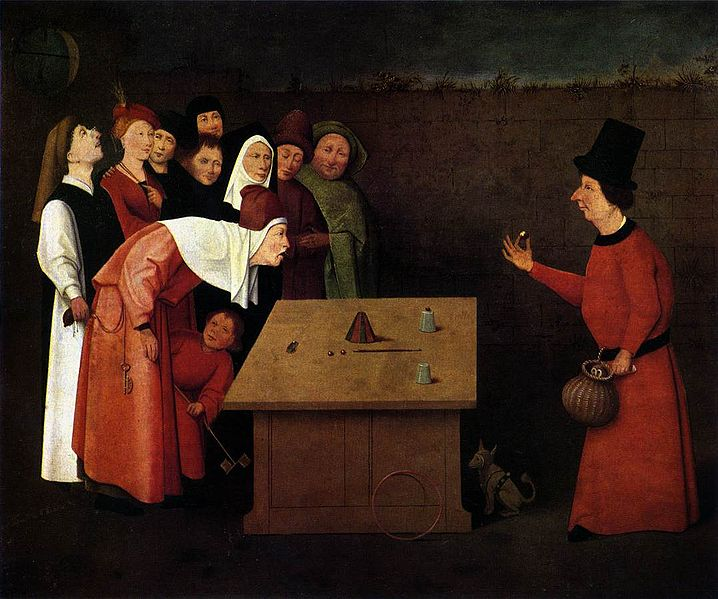
\includegraphics[scale=2.5]{symbolic/2_assembly/718px-Conjurer_Bosch.jpg}
\caption{Hieronymus Bosch -- The Conjurer}
\end{figure}

Again, we can build equivalent function which can take both numerical variables and Expr() objects.
We also extend Expr() class to support many arithmetical and boolean operations.
Also, Expr() methods would take both Expr() objects on input and integer values.

\lstinputlisting{symbolic/2_assembly/1.py}

I run it:

\begin{lstlisting}
((((initial_ECX&65280)|(initial_ECX<<16))<<8)|(((initial_ECX&16711680)|(initial_ECX>>16))>>8))
\end{lstlisting}

Now this is something more readable, however, a bit LISPy at first sight.
In fact, this is a function which change endianness in 32-bit word.

By the way, my Toy Decompiler can do this job as well, but operates on \ac{AST} instead
of plain strings: \ref{toy_decompiler}.

\subsubsection{Fast Fourier transform}

I've found one of the smallest possible FFT implementations on \href{https://www.reddit.com/r/Python/comments/1la4jp/understanding_the_fft_algorithm_with_python/}{reddit}:

\lstinputlisting{symbolic/3_FFT/FFT.py}

Just interesting, what value has each element on output?

\lstinputlisting{symbolic/3_FFT/FFT_symb.py}

FFT() function left almost intact, the only thing I added: complex value is converted into string and then
Expr() object is constructed.

\lstinputlisting{symbolic/3_FFT/res1.txt}

We can see subexpressions in form like $x^0$ and $x^1$.
We can eliminate them, since $x^0=1$ and $x^1=x$.
Also, we can reduce subexpressions like $x \cdot 1$ to just $x$.

\begin{lstlisting}
    def __mul__(self, other):
        op1=self.s
        op2=self.convert_to_Expr_if_int(other).s

        if op1=="1":
            return Expr(op2)
        if op2=="1":
            return Expr(op1)

        return Expr("(" + op1 + "*" + op2 + ")")

    def __pow__(self, other):
        op2=self.convert_to_Expr_if_int(other).s
        if op2=="0":
            return Expr("1")
        if op2=="1":
            return Expr(self.s)

        return Expr("(" + self.s + "**" + op2 + ")")
\end{lstlisting}

\lstinputlisting{symbolic/3_FFT/res2.txt}

\subsubsection{Cyclic redundancy check}

I've always been wondering, which input bit affects which bit in the final CRC32 value.

From the \ac{CRC} theory (good and concise introduction:
\url{http://web.archive.org/web/20161220015646/http://www.hackersdelight.org/crc.pdf}
) we know that \ac{CRC} is shifting register with taps.

We will track each bit rather than byte or word, which is highly inefficient, but serves our purpose better:

\lstinputlisting{symbolic/4_CRC/1.py}

Here are expressions for each CRC32 bit for 1-byte buffer:

\lstinputlisting{symbolic/4_CRC/1byte.txt}

For larger buffer, expressions gets increasing exponentially.
This is 0th bit of the final state for 4-byte buffer:

\begin{lstlisting}
state 0=((((((((((((((in_0_0^1)^(in_0_1^1))^(in_0_2^1))^(in_0_4^1))^(in_0_5^1))^(in_0_7^(1^(in_0_1^1))))^
(in_1_0^(1^(in_0_2^1))))^(in_1_2^(((1^(in_0_0^1))^(in_0_1^1))^(in_0_4^1))))^(in_1_3^(((1^(in_0_1^1))^
(in_0_2^1))^(in_0_5^1))))^(in_1_4^(((1^(in_0_2^1))^(in_0_3^1))^(in_0_6^(1^(in_0_0^1))))))^(in_2_0^((((1^
(in_0_0^1))^(in_0_6^(1^(in_0_0^1))))^(in_0_7^(1^(in_0_1^1))))^(in_1_2^(((1^(in_0_0^1))^(in_0_1^1))^(in_0_4^
1))))))^(in_2_6^(((((((1^(in_0_0^1))^(in_0_1^1))^(in_0_2^1))^(in_0_6^(1^(in_0_0^1))))^(in_1_4^(((1^(in_0_2^1))^
(in_0_3^1))^(in_0_6^(1^(in_0_0^1))))))^(in_1_5^(((1^(in_0_3^1))^(in_0_4^1))^(in_0_7^(1^(in_0_1^1))))))^
(in_2_0^((((1^(in_0_0^1))^(in_0_6^(1^(in_0_0^1))))^(in_0_7^(1^(in_0_1^1))))^(in_1_2^(((1^(in_0_0^1))^(in_0_1^1))^
(in_0_4^1))))))))^(in_2_7^(((((((1^(in_0_1^1))^(in_0_2^1))^(in_0_3^1))^(in_0_7^(1^(in_0_1^1))))^(in_1_5^(((1^
(in_0_3^1))^(in_0_4^1))^(in_0_7^(1^(in_0_1^1))))))^(in_1_6^(((1^(in_0_4^1))^(in_0_5^1))^(in_1_0^(1^(in_0_2^
1))))))^(in_2_1^((((1^(in_0_1^1))^(in_0_7^(1^(in_0_1^1))))^(in_1_0^(1^(in_0_2^1))))^(in_1_3^(((1^(in_0_1^1))^
(in_0_2^1))^(in_0_5^1))))))))^(in_3_2^(((((((((1^(in_0_1^1))^(in_0_2^1))^(in_0_4^1))^(in_0_5^1))^(in_0_6^(1^
(in_0_0^1))))^(in_1_2^(((1^(in_0_0^1))^(in_0_1^1))^(in_0_4^1))))^(in_2_0^((((1^(in_0_0^1))^(in_0_6^(1^(in_0_0^
1))))^(in_0_7^(1^(in_0_1^1))))^(in_1_2^(((1^(in_0_0^1))^(in_0_1^1))^(in_0_4^1))))))^(in_2_1^((((1^(in_0_1^1))^
(in_0_7^(1^(in_0_1^1))))^(in_1_0^(1^(in_0_2^1))))^(in_1_3^(((1^(in_0_1^1))^(in_0_2^1))^(in_0_5^1))))))^(in_2_4^
(((((1^(in_0_0^1))^(in_0_4^1))^(in_1_2^(((1^(in_0_0^1))^(in_0_1^1))^(in_0_4^1))))^(in_1_3^(((1^(in_0_1^1))^
(in_0_2^1))^(in_0_5^1))))^(in_1_6^(((1^(in_0_4^1))^(in_0_5^1))^(in_1_0^(1^(in_0_2^1))))))))))
\end{lstlisting}

Expression for the 0th bit of the final state for 8-byte buffer has length of $\approx 350KiB$,
which is, of course, can be reduced
significantly (because this expression is basically XOR tree), but you can feel the weight of it.

Now we can process this expressions somehow to get a smaller picture on what is affecting what.
Let's say, if we can find ``in\_2\_3'' substring in expression, this means that 3rd bit of 2nd byte of input
affects this expression.
But even more than that: since this is XOR tree (i.e., expression consisting only of XOR operations),
if some input variable is occurring twice, it's \textit{annihilated}, since $x \oplus x=0$.
More than that: if a vairable occurred even number of times (2, 4, 8, etc), it's annihilated, but left if it's occurred
odd number of times (1, 3, 5, etc).

\begin{lstlisting}
    for i in range(32):
        #print "state %d=%s" % (i, state[31-i])
        sys.stdout.write ("state %02d: " % i)
        for byte in range(BYTES):
            for bit in range(8):
                s="in_%d_%d" % (byte, bit)
                if str(state[31-i]).count(s) & 1:
                    sys.stdout.write ("*")
                else:
                    sys.stdout.write (" ")
        sys.stdout.write ("\n")
\end{lstlisting}

( \url{https://github.com/dennis714/SAT_SMT_article/blob/master/symbolic/4_CRC/2.py} )

Now this how each bit of 1-byte input buffer affects each bit of the final CRC32 state:

\lstinputlisting{symbolic/4_CRC/1byte_tbl.txt}

This is 8*8=64 bits of 8-byte input buffer:

\lstinputlisting{symbolic/4_CRC/8byte_tbl.txt}

\subsubsection{Linear congruential generator}

This is popular \ac{PRNG} from OpenWatcom \ac{CRT} library: \url{https://github.com/open-watcom/open-watcom-v2/blob/d468b609ba6ca61eeddad80dd2485e3256fc5261/bld/clib/math/c/rand.c}.

What expression it generates on each step?

\lstinputlisting{symbolic/5_LCG/LCG.py}

\lstinputlisting{symbolic/5_LCG/1.txt}

Now if we once got several values from this PRNG, like 4583, 16304, 14440, 32315, 28670, 12568..., how would we
recover the initial seed?
The problem in fact is solving a system of equations:

\begin{lstlisting}
((((initial_seed*1103515245)+12345)>>16)&32767)==4583
((((((initial_seed*1103515245)+12345)*1103515245)+12345)>>16)&32767)==16304
((((((((initial_seed*1103515245)+12345)*1103515245)+12345)*1103515245)+12345)>>16)&32767)==14440
((((((((((initial_seed*1103515245)+12345)*1103515245)+12345)*1103515245)+12345)*1103515245)+12345)>>16)&32767)==32315
\end{lstlisting}

As it turns out, Z3 can solve this system correctly using only two equations:

\lstinputlisting{symbolic/5_LCG/Z3_solve.py}

\begin{lstlisting}
[x = 11223344]
\end{lstlisting}

(Though, it takes $\approx 20$ seconds on my ancient Intel Atom netbook.)

\subsubsection{Path constraint}

How to get weekday from UNIX timestamp?

\begin{lstlisting}
#!/usr/bin/env python

input=...
SECS_DAY=24*60*60
dayno = input / SECS_DAY
wday = (dayno + 4) % 7
if wday==5:
    print "Thanks God, it's Friday!"
\end{lstlisting}

Let's say, we should find a way to run the block with print() call in it.
What input value should be?

First, let's build expression of $wday$ variable:

\lstinputlisting{symbolic/6_TGIF/TGIF.py}

\begin{lstlisting}
(((input/86400)+4)%7)
\end{lstlisting}

In order to execute the block, we should solve this equation: $((\frac{input}{86400}+4) \equiv 5 \mod 7$.

So far, this is easy task for Z3:

\lstinputlisting{symbolic/6_TGIF/Z3_solve.py}

\begin{lstlisting}
[x = 86438]
\end{lstlisting}

This is indeed correct UNIX timestamp for Friday:

\begin{lstlisting}
% date --date='@86438'
Fri Jan  2 03:00:38 MSK 1970
\end{lstlisting}

Though the date back in year 1970, but it's still correct!

This is also called ``path constraint'', i.e., what constraint must be satisified to execute specific block?
Several tools has ``path'' in their names, like
``pathgrind'', 
\href{http://babelfish.arc.nasa.gov/trac/jpf/wiki/projects/jpf-symbc}{Symbolic PathFinder}, CodeSurfer Path Inspector, etc.

Like the shell game, this task is also often encounters in practice.
You can see that something dangerous can be executed inside some basic block and you're trying to deduce,
what input values can cause execution of it.
It may be buffer overflow, etc.
Such input values are sometimes also called ``inputs of death''.

Many crackmes are solved in this way, all you need is find a path into block which prints ``key is correct''
or something like that.

We can extend this tiny example:

\begin{lstlisting}
input=...
SECS_DAY=24*60*60
dayno = input / SECS_DAY
wday = (dayno + 4) % 7
print wday
if wday==5:
    print "Thanks God, it's Friday!"
else:
    print "Got to wait a little"
\end{lstlisting}

Now we have two blocks: for the first we should solve this equation: $((\frac{input}{86400}+4) \equiv 5 \mod 7$.
But for the second we should solve inverted equation: $((\frac{input}{86400}+4) \not\equiv 5 \mod 7$.
By solving these equations, we will find two paths into both blocks.

KLEE (or similar tool) tries to find path to each [basic] block and produces ``ideal'' unit test.
Hence, KLEE can find a path into the block which crashes everything, or reporting about correctness of the input
key/license, etc.
Surprisingly, KLEE can find backdoors in the very same manner.

KLEE is also called ``KLEE Symbolic Virtual Machine'' -- by that its creators mean that the KLEE is \ac{VM} which executes a code symbolically rather than numerically (like usual \ac{CPU}).

\subsubsection{Division by zero}

If division by zero is unwrapped by sanitizing check, and exception isn't caught, it can crash process.

Let's calculate simple expression $\frac{x}{2y + 4z - 12}$.
We can add a warning into \TT{\_\_div\_\_} method:

\lstinputlisting{symbolic/7_div/1.py}

\dots so it will report about dangerous states and conditions:

\begin{lstlisting}
warning: division by zero if (((y*2)+(z*4))-12)==0
(x/(((y*2)+(z*4))-12))
\end{lstlisting}

This equation is easy to solve, let's try Wolfram Mathematica this time:

\begin{lstlisting}
In[]:= FindInstance[{(y*2 + z*4) - 12 == 0}, {y, z}, Integers]
Out[]= {{y -> 0, z -> 3}}
\end{lstlisting}

These values for $y$ and $z$ can also be called ``inputs of death''.

\subsubsection{Merge sort}

How merge sort works?
I have copypasted Python code from rosettacode.com almost intact:

\lstinputlisting{symbolic/8_sorting/1.py}

But here is a function which compares elements.
Obviously, it wouldn't work correctly without it.

So we can track both expression for each element and numerical value.
Both will be printed finally.
But whenever values are to be compared, only numerical parts will be used.

Result:

\lstinputlisting{symbolic/8_sorting/result.txt}

\subsubsection{Extending Expr class}

This is somewhat senseless, nevertheless, it's easy task to extend my Expr class to support \ac{AST} instead of
plain strings.
It's also possible to add folding steps (like I demonstrated in Toy Decompiler: \ref{toy_decompiler}).
Maybe someone will want to do this as an exercise.
By the way, the toy decompiler can be used as simple symbolic engine as well,
just feed all the instructions to it and it will track contents of each register.

\subsubsection{Conclusion}

For the sake of demonstration, I made things as simple as possible.
But reality is always harsh and inconvenient, so all this shouldn't be taken as a silver bullet.

The files used in this part: \url{https://github.com/dennis714/SAT_SMT_article/tree/master/symbolic}.

